\documentclass[8pt,executivepaper]{article}
\usepackage[utf8]{inputenc}
\usepackage[spanish]{babel}
\usepackage{amsmath}
\usepackage{amsfonts}
\usepackage{amssymb}
\usepackage{graphics}
\usepackage{graphicx}
\usepackage[left=1cm,right=1cm,top=2cm,bottom=2cm]{geometry}
\usepackage{imakeidx}
\makeindex[columns=3, title=Alphabetical Index, intoc]
\usepackage{listings}
\usepackage{xcolor}
\usepackage{multicol}
\usepackage{changepage}
\usepackage{float}
\usepackage{cite}
\usepackage{url}
\usepackage{hyperref}
\usepackage{pdfpages}
\usepackage{pgf,pgffor}

\definecolor{codegreen}{rgb}{0,0.6,0}
\definecolor{codegray}{rgb}{0.5,0.5,0.5}
\definecolor{codepurple}{rgb}{0.58,0,0.82}
\definecolor{backcolour}{rgb}{0.95,0.95,0.92}
\lstdefinestyle{mystyle}{
    backgroundcolor=\color{backcolour},
    commentstyle=\color{codegreen},
    keywordstyle=\color{magenta},
    numberstyle=\tiny\color{codegray},
    stringstyle=\color{codepurple},
    basicstyle=\ttfamily\footnotesize,
    breakatwhitespace=false,
    breaklines=true,
    captionpos=b,
    keepspaces=true,
    numbers=left,
    numbersep=5pt,
    showspaces=false,
    showstringspaces=false,
    showtabs=false,
    tabsize=3
}
\lstset{style=mystyle}
\author{González Pardo Adrian}
\date{Mayo 2020}
\title{Reporte de practica 11}
\newcommand\tab[1][1cm]{\hspace*{#1}}
\begin{document}
\maketitle
\section{Código fuente:}
\subsection{Memoria de programa}
\begin{center}
  \lstinputlisting[language=VHDL]{vhd/pc.vhd}
\end{center}
\subsection{Stack}
\begin{center}
  \lstinputlisting[language=VHDL]{vhd/pila.vhd}
\end{center}
\subsection{Unión para la arquitectura}
\begin{center}
  \lstinputlisting[language=VHDL]{vhd/pila-pc.vhd}
\end{center}
\section{Test-Bench:}
\begin{center}
  \lstinputlisting[language=VHDL]{vhd/pila_TB.vhd}
\end{center}
\section{Archivos de entrada y salida}
\subsection{Entrada}
\begin{center}
  \lstinputlisting{sources/in.txt}
\end{center}
\clearpage
\subsection{Salida}
\begin{center}
  \lstinputlisting{sources/out.txt}
\end{center}
\section{Diagrama RTL}
\begin{center}
  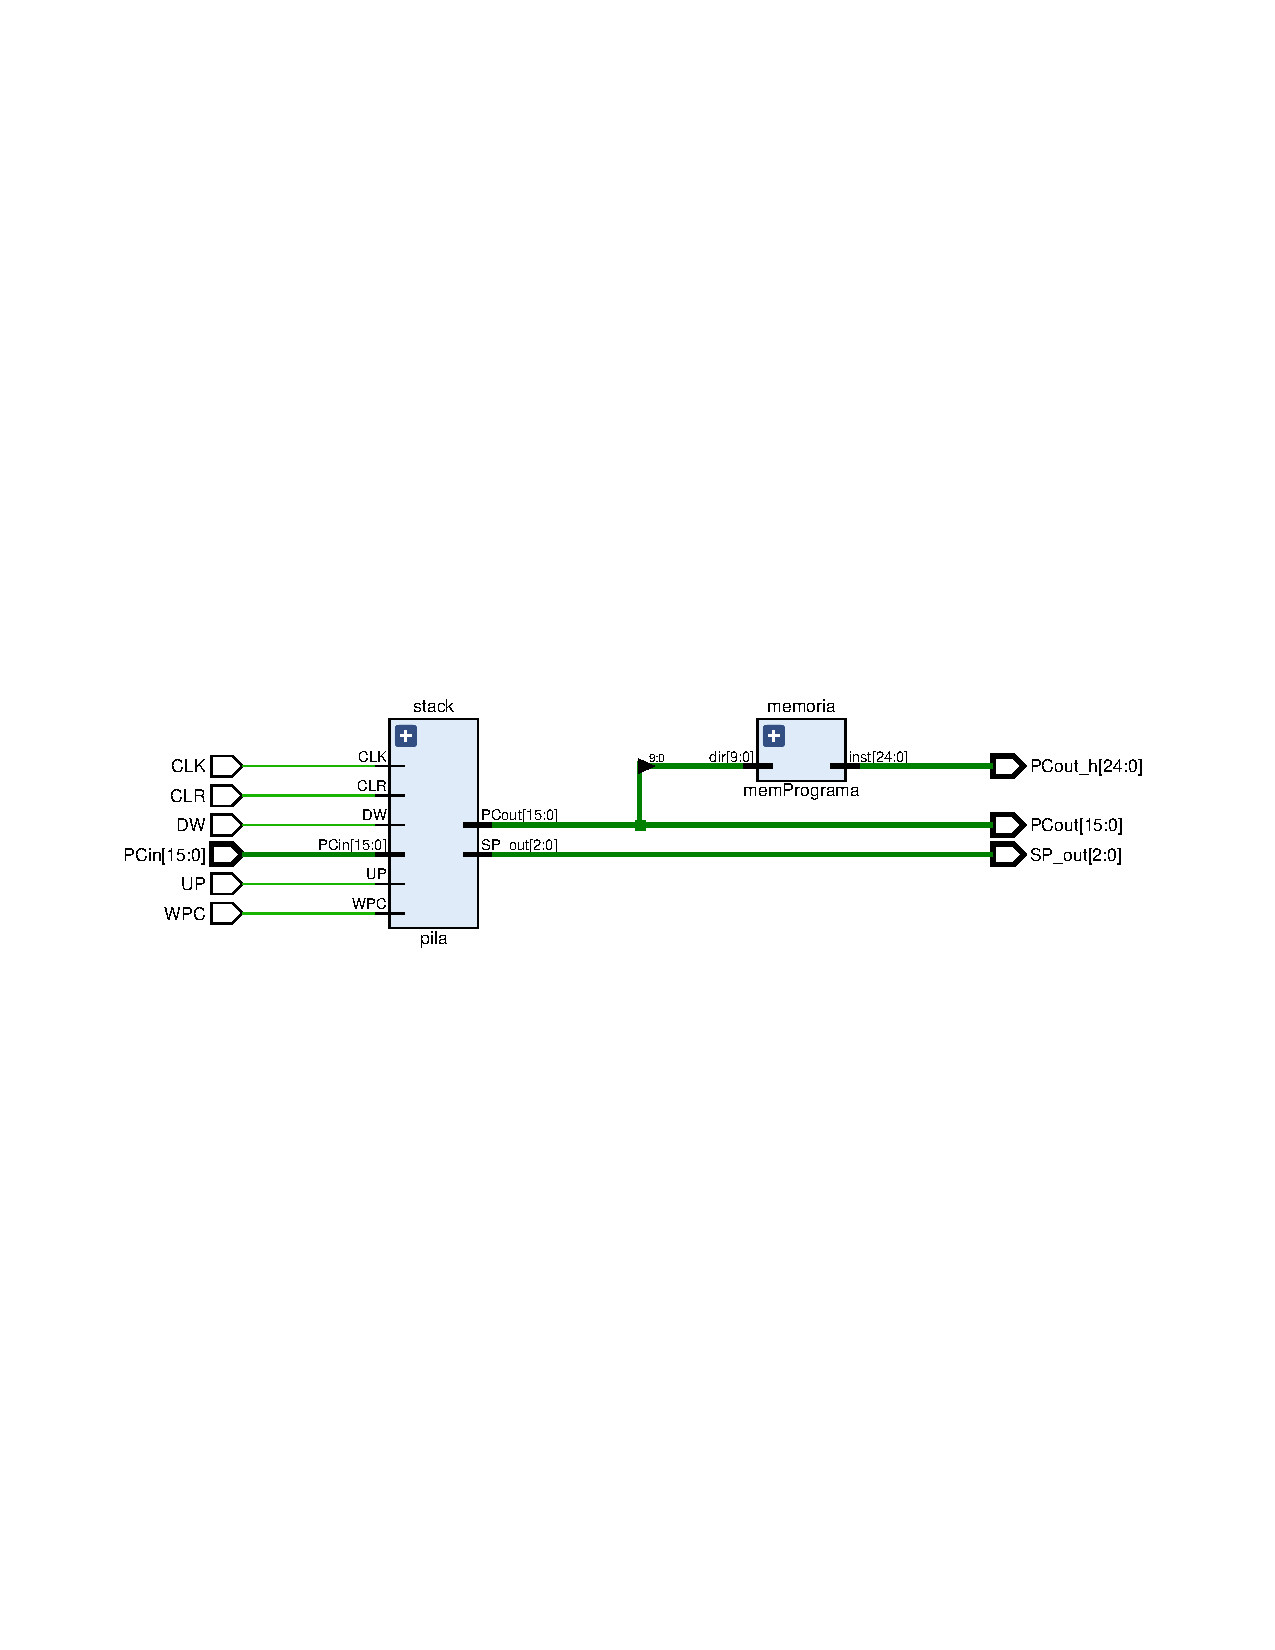
\includegraphics[scale=0.65]{sources/RTL.pdf}
\end{center}
\end{document}
